\newpage
\section{Einleitung}
\begin{wrapfigure}[16]{r}{8.5cm}
	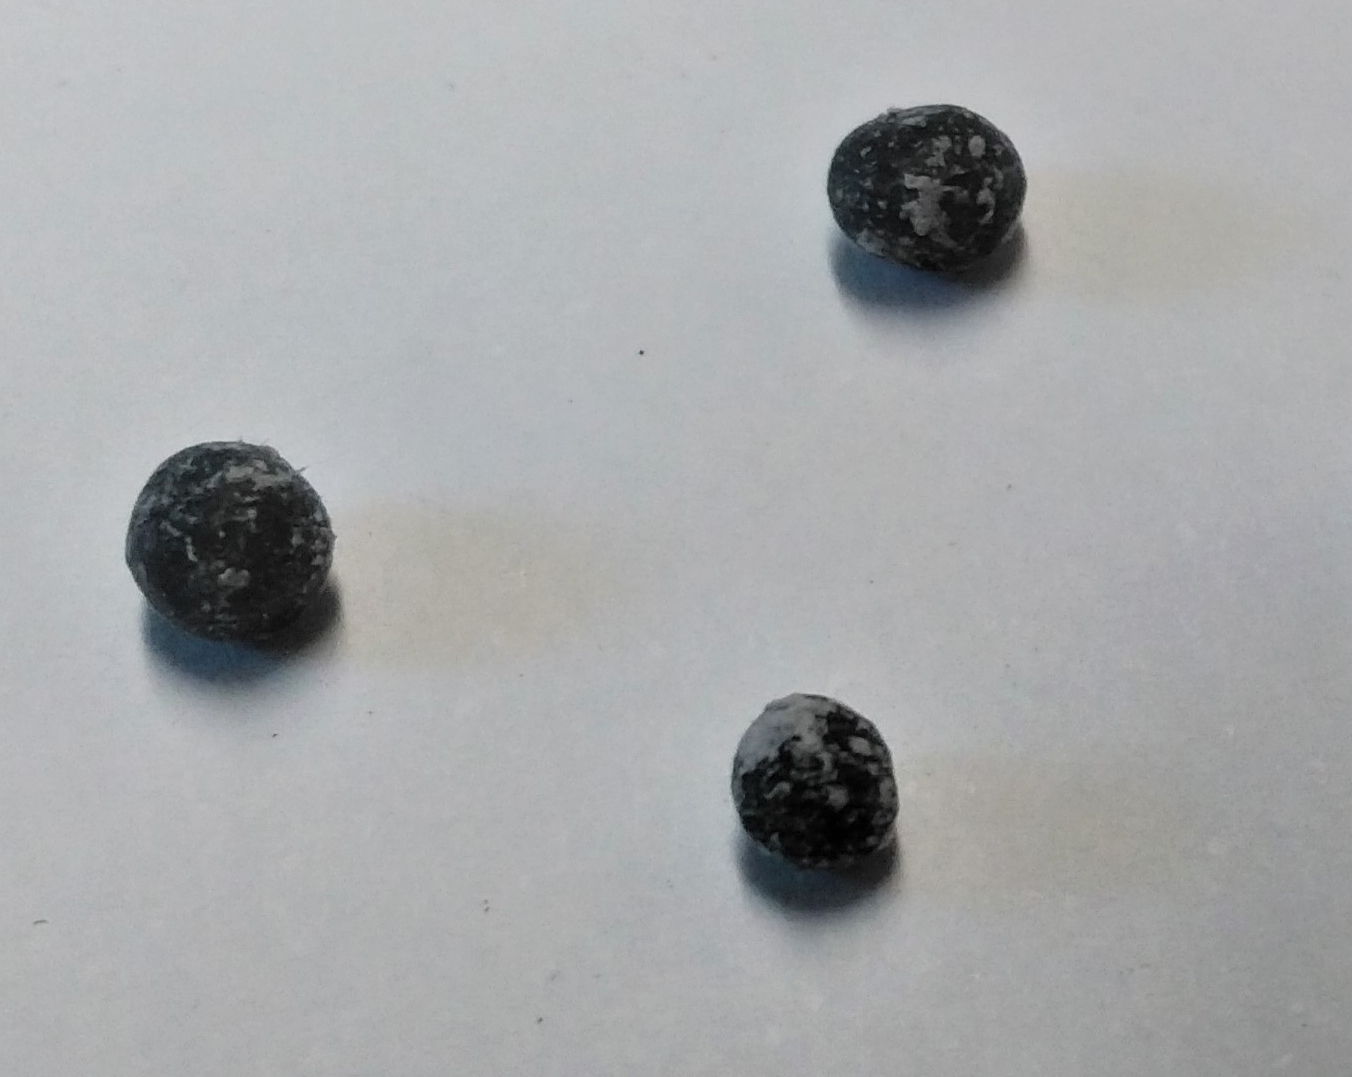
\includegraphics[scale=0.18]{Illustrationen/3-Einleitung/nemacaps.jpg}
	\caption{NemaCaps}
	\label{fig:nemacaps}
\end{wrapfigure}
\textit{(ygu)} Die Firma MCC Laboratoire Meiners GmbH ist in der Herstellung von Mikroverkapselungen tätig. Neben der Pharma- und Kosmetikbranche werden Mikroverkapselungen auch in der Landwirtschaft eingesetzt. Für diese Branche entwickelt MCC Laboratoire Meiners GmbH Kapseln, sogenannte NemaCaps, welche in der biologischen Schädlingsbekämpfung eingesetzt werden. Ein NemaCap beinhaltet mehrere tausend Fadenwürmer (Nematoden). Neben Nematoden ist der Kapsel ein Schlafmittel beigemischt, sodass die Fadenwürmer schlafend gestellt sind. 
\newline
NemaCaps werden im Erdreich eingesetzt, wobei sie im Wurzelbereich der zu schützenden Pflanze platziert werden. Durch das Begiessen der Pflanze oder den Regen wird das Schlafmittel verdünnt und die Nematoden werden aktiv. Die Hülle der Kapseln besteht aus \textbf{\textit{XYZ}} welches elastische Eigenschaften besitzt. Dies ist Voraussetzung, dass die Nematoden nach dem Aufwachen die Kapsel durchbrechen können.\newline
In ihrer natürlichen Umgebung angelangt stossen die Fadenwürmer nun zufällig auf Larven von Schädlingen. Gemäss dem Nationalen Forschungsprogramm 68 [nachfolgend NFP 68]\cite{nfp} dringen die Nematoden durch die Körperöffnungen der Larven ein (Siehe Abb.  \ref{fig:zyklus_Nematoden}, Punkt 3). im Körper der Larve angelangt, setzen die Fadenwürmer dort Bakterien frei (Punkt 1 in Abb.  \ref{fig:zyklus_Nematoden}). Diese Infektion führt innerhalb von 1-2 Tagen zum Tod des Insekts \cite{e-nema}. Die Nematoden vermehren sich in den Larven bis diese komplett aufgezehrt ist \cite{nematoden}. Anschliessend verlassen die Nematoden den Kadaver und befallen weitere Larven. So beginnt der Kreislauf von Neuem (Punkt 2 in Abb.  \ref{fig:zyklus_Nematoden}).
\newline

\begin{wrapfigure}[10]{r}{7cm}
	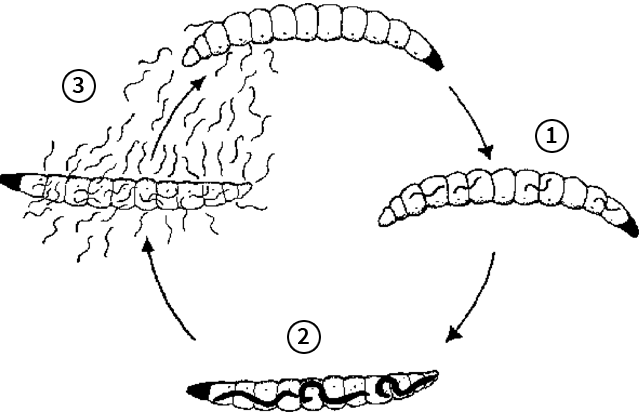
\includegraphics[scale=0.4]{Illustrationen/3-Einleitung/zyklus_nematoden.png}
\caption{Bekämpfung einer Larve durch Nematoden \protect\cite{e-nema}}
\label{fig:zyklus_Nematoden}
\end{wrapfigure}

	
Nematoden bieten speziell in der Bekämpfung gegen Wurzelschädlinge eine wirksame Alternative zu Pestiziden an. Pestizide können im Wurzelbereich weniger gezielt eingesetzt werden \cite{nfp}. Die Überlegenheit der Nematoden (im Wurzelbereich anhängen?) will man mit NemaCaps nutzen. Durch die Kapselung ist eine gezielte Platzierung sowie Dosierung von Nematoden möglich. Ein weiterer Vorteil der Kapselung ist die verbesserte Handhabung. Die einfache Lagerung sowie der Transport von Fadenwürmer wird möglich.  Zudem verlängert die Verwendung von Schlafmittel die Haltbarkeit der Nematoden. Diese Vorteile unterstreichen das Potential von NemaCaps, der biologischen Alternative von Pestiziden (Ist dieser Satz notwendig?).
